%-------------------------------------------------------------------------------
\section{Experiments}
\label{chap1-sec:experiments}
%-------------------------------------------------------------------------------

% We conducted experiments to evaluate our proposed algorithms. 
% In particular, we 
Based on our theoretical results in Section~\ref{chap1-sec:algorithms}, we would like to pose the following questions:
\begin{itemize}
    \item For triangle counts, how much does the two-rounds interaction help over a single round in practice?
    \item What is the privacy-utility trade-off 
    %for subgraph counts in the local model 
    of our LDP algorithms 
    (i.e., how beneficial are our LDP algorithms)?
    %\item Is it possible to accurately estimate triangle counts and $k$-star counts in the local model?
\end{itemize}
We conducted experiments to answer to these questions. 

\subsection{Experimental Set-up}
\label{chap1-sub:setup}
% We conducted experiments to evaluate our proposed algorithms. 
% In our experiments, 
We used the following two large-scale datasets:

\smallskip
% \noindent{\textbf{Remark.}}~~
\noindent{\textbf{IMDB.}}~~The Internet Movie Database (denoted by \IMDB{}) 
% was used for the Graph Drawing 2005 contest 
\cite{IMDB_GD05} 
% . It 
includes a bipartite graph between $896308$ actors and $428440$ movies. 
% where an edge between an actor and a movie represents that the actor participated in the movie. 
% We assumed $896308$ actors as users ($n=896308$). 
We assumed actors as users. 
From the bipartite graph, we extracted 
% an adjacency matrix $\bmA=(a_{ij})$, where $a_{ij} = 1$ 
% a graph $G=(V,E)$ with $896308$ nodes, where node $v_i$ represents the $i$-th actor and edge $(v_i, v_j) \in E$ represents that actors $v_i$ and $v_j$ have played in the same movie. 
a graph $G^*$ with $896308$ nodes (actors), where an edge between two actors represents that they have played in the same movie. 
There are $57064358$ edges in $G^*$, and the average degree in $G^*$ is $63.7$ $(=\frac{57064358}{896308})$.

\smallskip
\noindent{\textbf{Orkut.}}~~The 
% Orkut is a social networking service operated by Google from $2004$ to $2014$. 
Orkut online social network dataset (denoted by \Orkut{})  \cite{snapnets} includes a graph $G^*$ with $3072441$ users and $117185083$ edges. 
The average degree in $G^*$ is $38.1$ $(=\frac{117185083}{3072441})$. 
Therefore, \Orkut{} is more sparse than \IMDB{} (whose average degree in $G^*$ is $63.7$). 
% Since the average degree is different between \IMDB{} and \Orkut{} (\Orkut{} is more sparse), we can 
% see the difference of the results.
% examine its effect on the results. 

\smallskip
For each dataset, we randomly selected $n$ users from the whole graph $G^*$, and extracted a graph $G=(V,E)$ with 
% the 
$n$ users. 
Then we estimated the number of triangles $f_\triangle(G)$, the number of $k$-stars $f_{k\star}(G)$, and the clustering coefficient ($=\frac{3 f_\triangle(G)}{f_{2\star}(G)}$) using $\epsilon$-edge LDP (or $\epsilon$-edge centralized DP) algorithms in Section~\ref{chap1-sec:algorithms}. 
Specifically, we used the following algorithms:

\smallskip
\noindent{\textbf{Algorithms for triangles.}}~~For algorithms for estimating $f_\triangle(G)$, we used the following three algorithms: 
(1) the RR (Randomized Response) with the empirical estimation method in the local model (i.e., \alg{LocalRR$_\triangle$} in Section~\ref{chap1-sub:non-interactive_triangles}), 
(2) the two-rounds algorithm in the local model (i.e., \alg{Local2Rounds$_\triangle$} in Section~\ref{chap1-sub:two_rounds}), and 
(3) the Laplacian mechanism in the centralized model (i.e., \alg{CentralLap$\triangle$} in Section~\ref{chap1-sub:non-interactive_triangles}).

\smallskip
\noindent{\textbf{Algorithms for $k$-stars.}}~~For algorithms for estimating $f_{k\star}(G)$, we used the following two algorithms: 
(1) the Laplacian mechanism in the local model (i.e., \alg{LocalLap$_k\star$} in Section~\ref{chap1-sub:non-interactive_k_stars}) and 
(2) the Laplacian mechanism in the centralized model (i.e., \alg{CentralLap$_k\star$} in Section~\ref{chap1-sub:non-interactive_k_stars}). 
% \alg{central (Lap)} for $k$-stars differs from \alg{central (Lap)} for triangles only in the sensitivity. 

\smallskip
For each algorithm, we evaluated the $l_2$ loss and the relative error (as described in Section~\ref{chap1-sub:graph_statistics}), while changing the values of $n$ and $\epsilon$. 
To stabilize the performance, we attempted $\gamma \in \nats$ ways to randomly select $n$ users from $G^*$, and averaged the utility value over all the $\gamma$ ways to randomly select $n$ users. 
When we changed $n$ from $1000$ to $10000$, we set $\gamma = 100$ because the variance was large. For other cases, we set $\gamma = 10$. 

In Appendix~\ref{chap1-sec:BAGraph}, 
we also report experimental results using artificial graphs based on the Barab\'{a}si-Albert model \cite{NetworkScience}.

\begin{figure}[t]
\centering
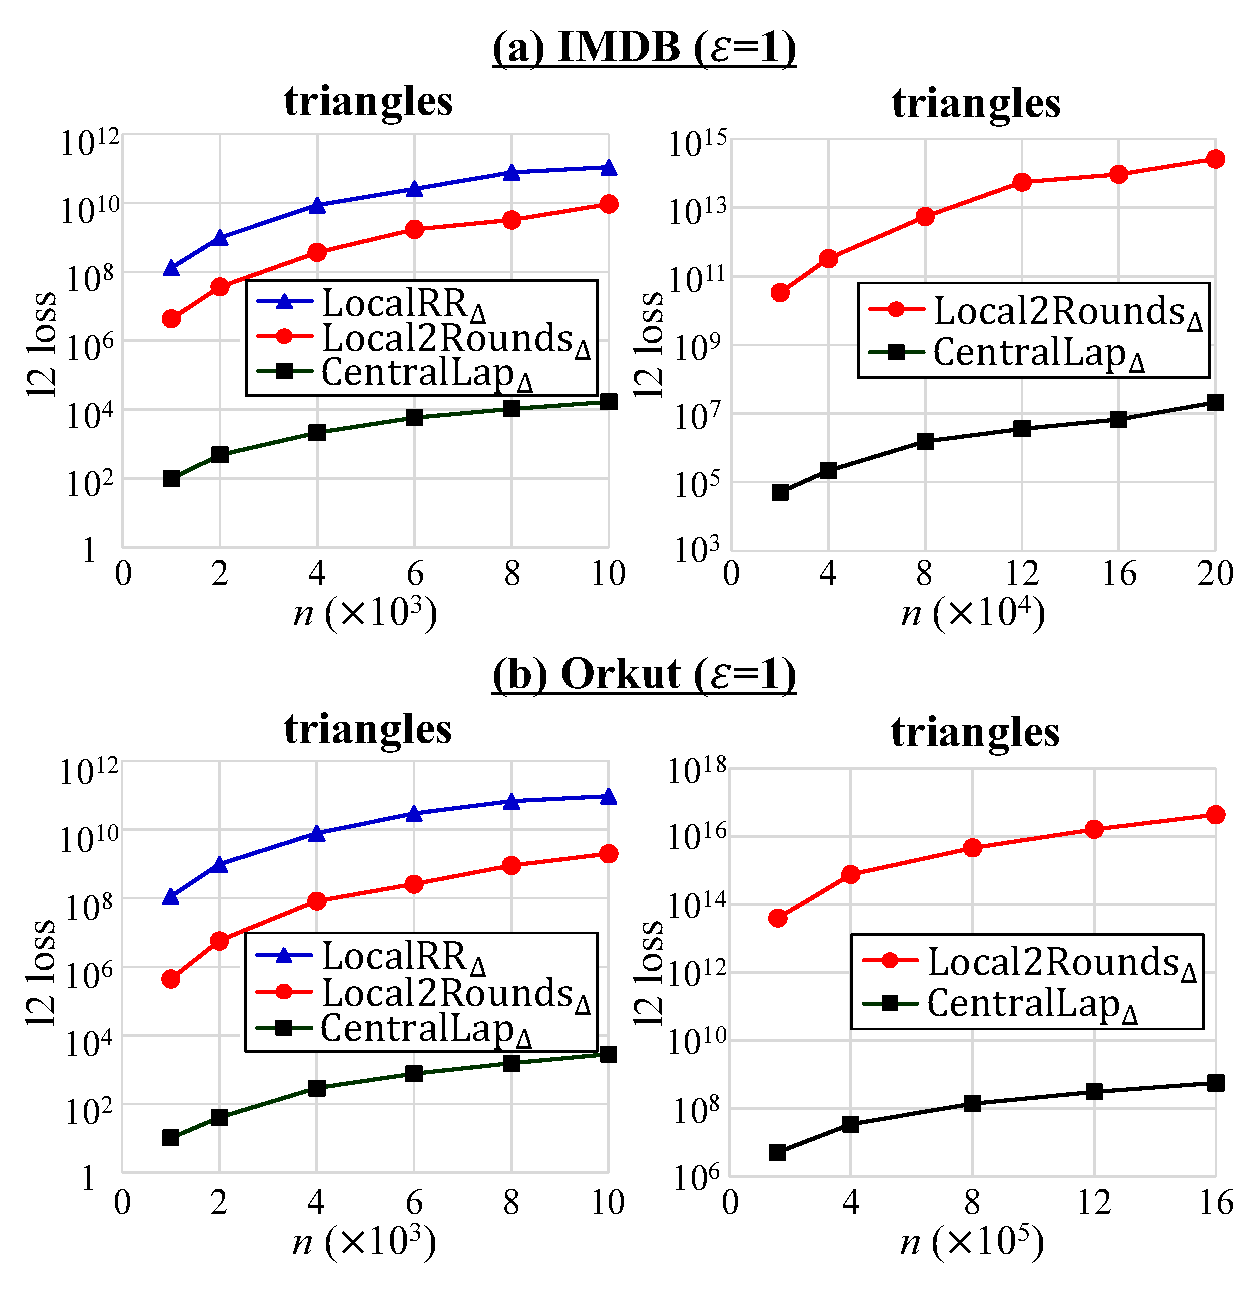
\includegraphics[width=0.99\linewidth]{fig/res1_n_l2loss_tri.pdf}

\caption[Relation between the number of users $n$ and the $l_2$ loss in triangle counts.]
{Relation between the number of users $n$ and the $l_2$ loss in triangle counts when $\epsilon = 1$ ($\epsilon_1 = \epsilon_2 = \frac{1}{2}$, $\td_{max} = d_{max}$). 
Here we do not evaluate \alg{LocalRR$_\triangle$} when $n > 10000$, because it is inefficient (see Section~\ref{chap1-sub:two_rounds} ``Time complexity'').}
\label{chap1-fig:res1_n_l2loss_tri}
\end{figure}

\begin{figure}[t]
\centering
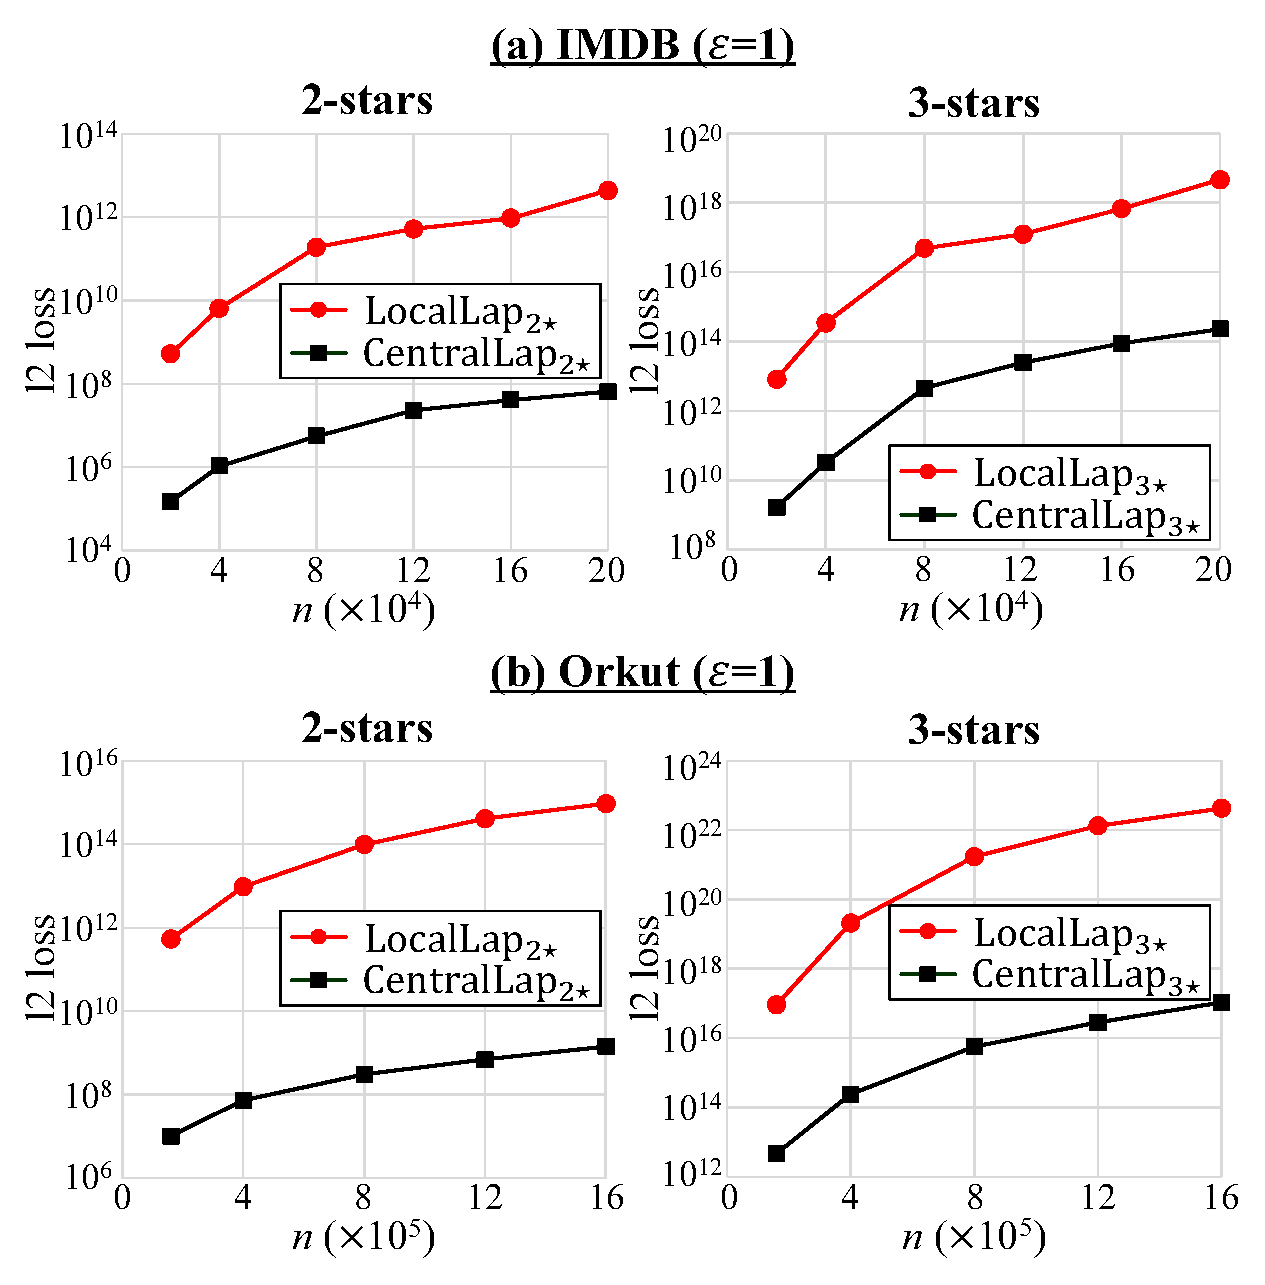
\includegraphics[width=0.99\linewidth]{fig/res1_n_l2loss_kst.pdf}

\caption[Relation between the number of users $n$ and the $l_2$ loss in $k$-star counts.]
{Relation between the number of users $n$ and the $l_2$ loss in $k$-star counts when $\epsilon=1$ ($\epsilon_1 = \epsilon_2 = \frac{1}{2}$, $\td_{max} = d_{max}$).}
\label{chap1-fig:res1_n_l2loss_kst}
\end{figure}

\subsection{Experimental Results}
\label{chap1-sub:results}
\noindent{\textbf{Relation between $n$ and the $l_2$ loss.}}~~We first evaluated the $l_2$ loss of the estimates of 
% the numbers of triangles ($f_\triangle(G)$), $2$-stars ($f_{2\star}(G)$), and $3$-stars ($f_{3\star}(G)$), 
$f_\triangle(G)$, 
% (triangle counts), 
$f_{2\star}(G)$, 
% ($2$-star counts), 
and $f_{3\star}(G)$ 
% ($3$-star counts) 
while changing the number of users $n$. 
Figures~\ref{chap1-fig:res1_n_l2loss_tri} and \ref{chap1-fig:res1_n_l2loss_kst} shows the results ($\epsilon=1$). 
Here 
% we changed $n$ from $1000$ to $200000$ in \IMDB{}, and from $1000$ to $1600000$ in \Orkut{}. 
% Note that 
we did not evaluate \alg{LocalRR$_\triangle$} when $n$ was larger than $10000$, because \alg{LocalRR$_\triangle$} was inefficient 
% (the time complexity of \alg{LocalRR$_\triangle$} is $O(n^3)$, as described in Section~\ref{chap1-sub:two_rounds}). 
(as described in Section~\ref{chap1-sub:two_rounds} ``Time complexity''). 
% In Figures~\ref{chap1-fig:res1_n_l2loss_tri} and \ref{chap1-fig:res1_n_l2loss_kst}, 
In \alg{Local2Rounds$_\triangle$}, we set $\epsilon_1 = \epsilon_2 = \frac{1}{2}$. 
% so that $\epsilon = \epsilon_1 + \epsilon_2 = 1$. 
% In \alg{Local2Rounds$_\triangle$},  \alg{CentralLap$_\triangle$}, \alg{LocalLap$_k\star$}, and \alg{CentralLap$_k\star$}, 
As for $\td_{max}$, 
we set $\td_{max} = d_{max}$ (i.e., we assumed that $d_{max}$ is publicly available and did not perform graph projection) 
% , 
because we want to examine how well our theoretical results hold in our experiments. 
% we added the Laplacian noise with the local sensitivity in \alg{Proposal}, \alg{central (Lap)}, and \alg{local (Lap)}. 
We also evaluate the effectiveness of the private calculation of $d_{max}$ at the end of Section~\ref{chap1-sub:results}. 

Figure~\ref{chap1-fig:res1_n_l2loss_tri} shows that \alg{Local2Rounds$_\triangle$} significantly outperforms \alg{LocalRR$_\triangle$}. 
% for estimating $f_\triangle(G)$. 
Specifically, the $l_2$ loss of \alg{Local2Rounds$_\triangle$} is smaller than that of \alg{LocalRR$_\triangle$} by a factor of about $10^2$. 
% and $10^2 \sim 10^3$ in \IMDB{} and \Orkut{}, respectively. 
The difference between \alg{Local2Rounds$_\triangle$} and \alg{LocalRR$_\triangle$} is larger in \Orkut{}. 
This is because \Orkut{} is more sparse, as described in Section~\ref{chap1-sub:setup}. 
For example, when $n=10000$, the maximum degree $d_{max}$ in $G$ was $73.5$ and $27.8$ on average in \IMDB{} and \Orkut{}, respectively. 
Recall that for a fixed $\epsilon$, 
the expected $l_2$ loss of \alg{Local2Rounds$_\triangle$} and \alg{LocalRR$_\triangle$} 
can be expressed as $O(nd_{max}^3)$ and $O(n^4)$, respectively. 
Thus \alg{Local2Rounds$_\triangle$} significantly outperforms \alg{LocalRR$_\triangle$}, especially in sparse graphs. 
% datasets. 

% Figures~\ref{chap1-fig:res1_n_l2loss_tri} and \ref{chap1-fig:res1_n_l2loss_kst} show that \alg{central (Lap)} provides the best performance, which is consistent with our theoretical results; i.e., 

Figures~\ref{chap1-fig:res1_n_l2loss_tri} and \ref{chap1-fig:res1_n_l2loss_kst} show that the $l_2$ loss is roughly consistent with 
our upper-bounds in terms of $n$. 
Specifically, 
\alg{LocalRR$_\triangle$}, 
\alg{Local2Rounds$_\triangle$},  \alg{CentralLap$_\triangle$}, 
\alg{LocalLap$_{k\star}$}, and 
\alg{CentralLap$_{k\star}$} achieve 
the expected $l_2$ loss of $O(n^4)$, $O(nd_{max}^3)$, $O(d_{max}^2)$, $O(nd_{max}^{2k-2})$, and $O(d_{max}^{2k-2})$, respectively. 
Here note that 
% the maximum degree $d_{max}$ increases roughly in proportion to $n$ (though $d_{max}$ is much smaller than $n$), 
each user's degree increases roughly in proportion to $n$ (though the degree is much smaller than $n$), 
as we randomly select $n$ users from the whole graph $G^*$. Assuming that $d_{max} = O(n)$,  Figures~\ref{chap1-fig:res1_n_l2loss_tri} and \ref{chap1-fig:res1_n_l2loss_kst} are roughly consistent with the upper-bounds. 
The figures also show the limitations of the local model in terms of the utility when compared to the centralized model.

% when we increase $n$ by a factor of $10$, 
% the $l_2$ loss in triangle counts increases by a factor of about $10^4$, $10^4$, $10^2$ in \alg{LocalRR$_\triangle$}, \alg{Local2Rounds$_\triangle$}, and \alg{central (Lap)}, respectively. 
% Therefore, the experimental results are roughly consistent with our theoretical results that the expected $l_2$ loss of \alg{LocalRR$_\triangle$}, \alg{Local2Rounds$_\triangle$}, and \alg{CentralLap$_\triangle$} is $O(n^4)$, $O(nd_{max}^3)$, and $O(d_{max}^2)$, respectively. 
% The same applies to $k$-star counts. 

\smallskip
\noindent{\textbf{Relation between $\epsilon$ and the $l_2$ loss.}}~~Next we evaluated the $l_2$ loss 
% of the estimates of $f_\triangle(G)$ (triangle counts) and $f_{2\star}(G)$ ($2$-star counts), 
when we changed the privacy budget $\epsilon$ in edge LDP. 
Figure~\ref{chap1-fig:res2_eps_l2loss} shows the results for triangles and $2$-stars ($n=10000$). 
% (the result of $3$-stars is similar to that of $2$-stars, and therefore we omit the result of $3$-stars). 
Here we omit the result of $3$-stars because it is similar to that of $2$-stars. 
In \alg{Local2Rounds$_\triangle$}, we set $\epsilon_1 = \epsilon_2 = \frac{\epsilon}{2}$. 

Figure~\ref{chap1-fig:res2_eps_l2loss} shows that the $l_2$ loss is roughly consistent with 
% the expected $l_2$ loss in 
% our theoretical analysis 
our upper-bounds in terms of $\epsilon$. 
For example, when we decrease $\epsilon$ from $0.4$ to $0.1$, the $l_2$ loss 
% in triangle counts 
increases by a factor of about $5000$, $200$, and $16$ for both the datasets in \alg{LocalRR$_\triangle$}, \alg{Local2Rounds$_\triangle$}, and \alg{CentralLap$_\triangle$}, respectively. 
% This is 
They are 
roughly consistent with our theoretical results 
that for small $\epsilon$, the expected $l_2$ loss of \alg{LocalRR$_\triangle$}, \alg{Local2Rounds$_\triangle$}, and \alg{CentralLap$_\triangle$} is  $O(\epsilon^{-6})$\footnote{We used $e^\epsilon \approx \epsilon + 1$ to derive the upper-bound of \alg{LocalRR$_\triangle$} for small $\epsilon$.}, $O(\epsilon^{-4})$, and $O(\epsilon^{-2})$, respectively. 
% The same applies to large $\epsilon$ (e.g., $\epsilon = 1$ or $2$). 

\begin{figure}[t]
\centering
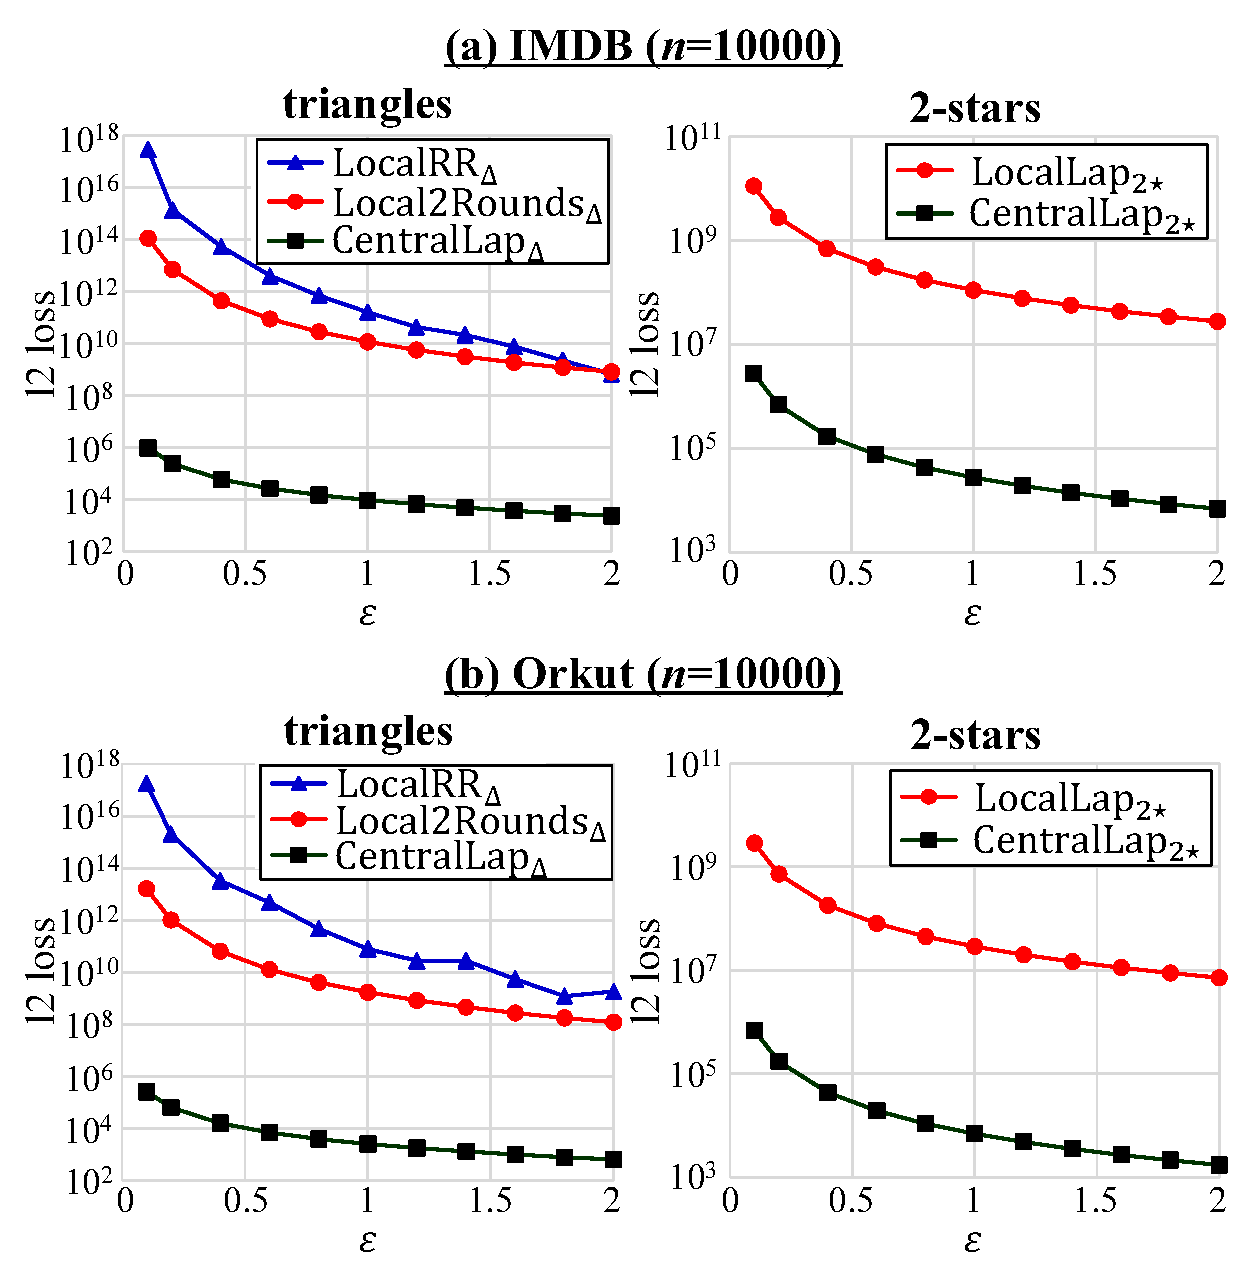
\includegraphics[width=0.99\linewidth]{fig/res2_eps_l2loss.pdf}

\caption[Relation between $\epsilon$ in edge LDP and the $l_2$ loss.]
{Relation between $\epsilon$ in edge LDP and the $l_2$ loss when $n=10000$ ($\epsilon_1 = \epsilon_2 = \frac{\epsilon}{2}$, $\td_{max} = d_{max}$).}
\label{chap1-fig:res2_eps_l2loss}
\end{figure}

\begin{figure}[t]
\centering
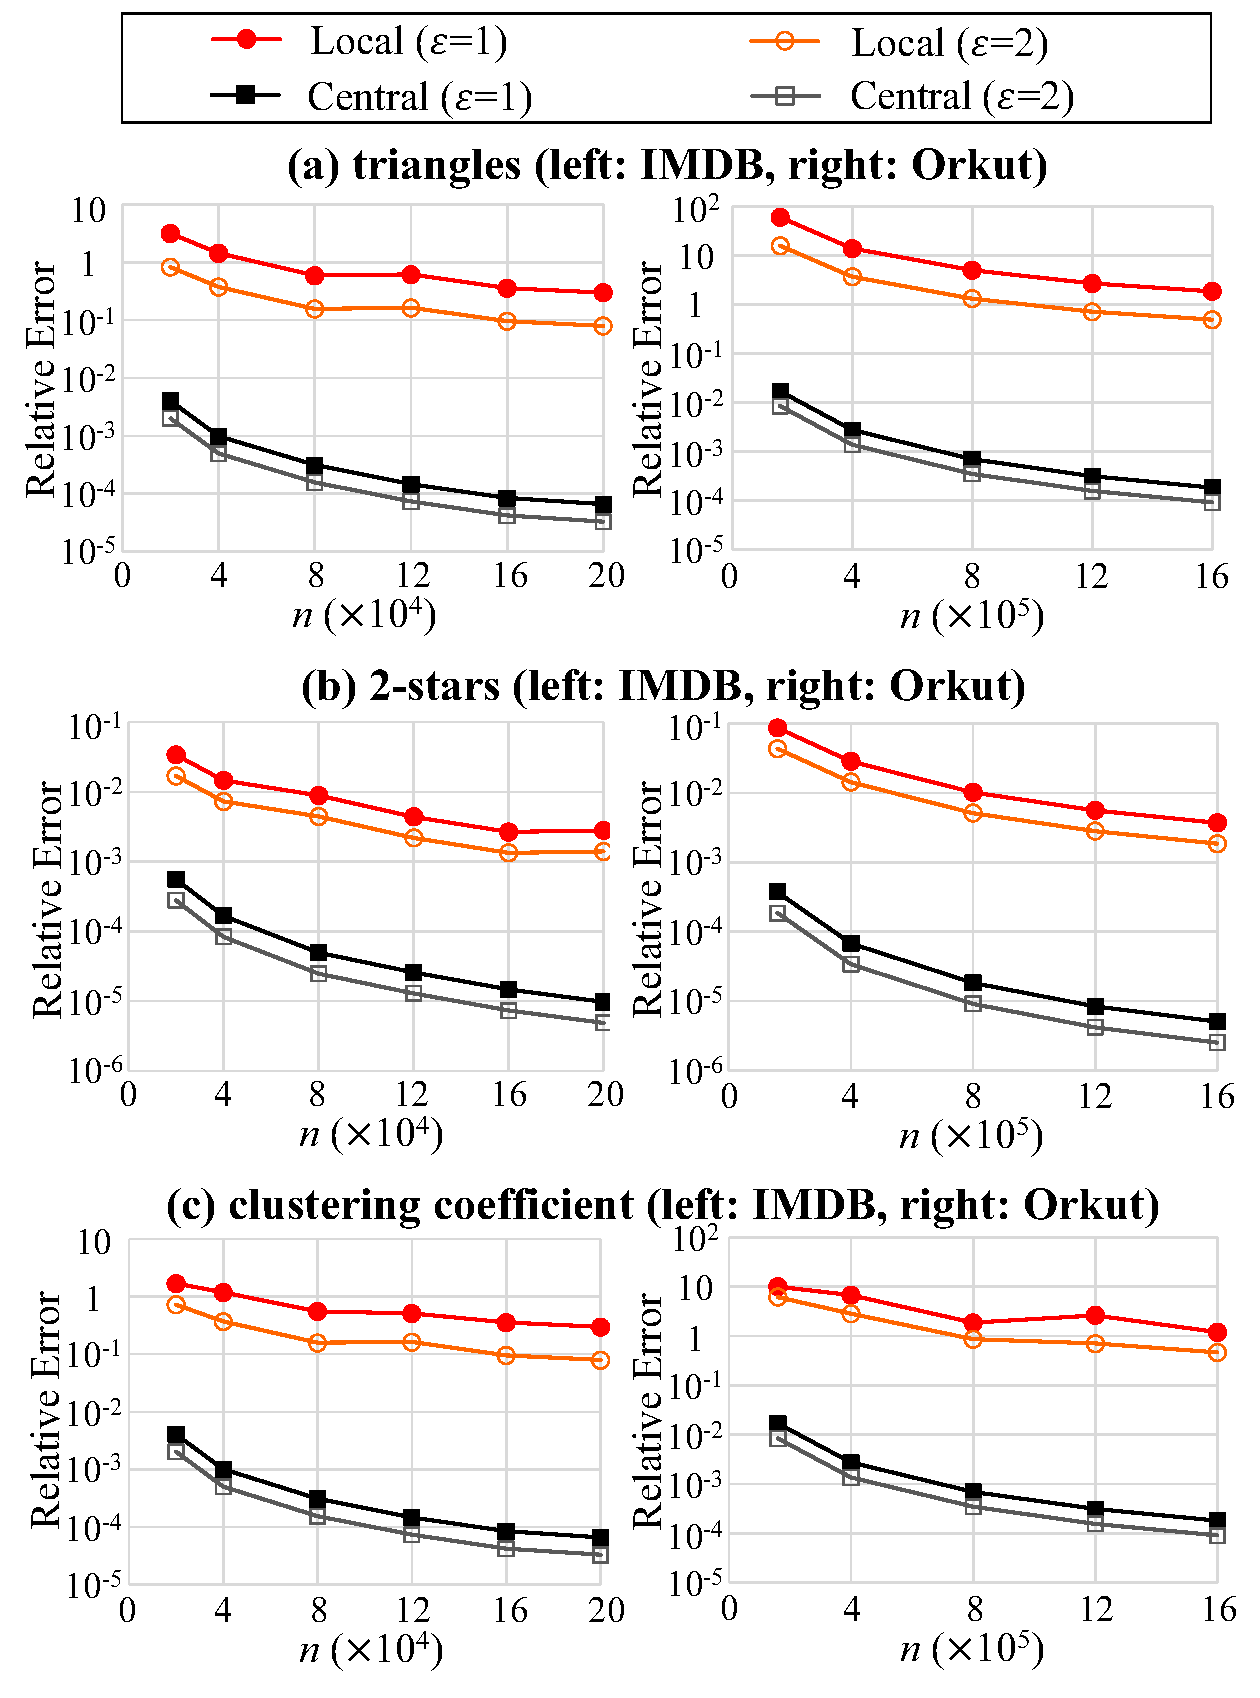
\includegraphics[width=0.99\linewidth]{fig/res3_n_relerr.pdf}

\caption[Relation between $n$ and the relative error.]{Relation between 
$n$ and the relative error. In the local model, we used \alg{Local2Rounds$_\triangle$} ($\epsilon = 1$ or $2$) and \alg{LocalLap$_k\star$} ($\epsilon = 1$ or $2$) for estimating triangle counts $f_\triangle(G)$ and $k$-star counts $f_{k\star}(G)$, respectively ($\td_{max} = d_{max}$).}
\label{chap1-fig:res3_n_relerr}
\end{figure}

Figure~\ref{chap1-fig:res2_eps_l2loss} also shows that 
\alg{Local2Rounds$_\triangle$} significantly outperforms \alg{LocalRR$_\triangle$} especially when $\epsilon$ is small, which is also consistent with our theoretical results. 
Conversely, the difference between \alg{LocalRR$_\triangle$} and \alg{Local2Rounds$_\triangle$} is small when $\epsilon$ is large. 
This is because when $\epsilon$ is large, the RR outputs the true value with high probability. 
For example, when 
% $\epsilon \geq 3$, 
$\epsilon \geq 5$, 
the RR outputs the true value with 
% $\frac{e^\epsilon}{e^\epsilon+1} > 0.95$. 
$\frac{e^\epsilon}{e^\epsilon+1} > 0.993$. 
% We also confirmed that when $\epsilon \geq 3$, the $l_2$ loss of \alg{LocalRR$_\triangle$} is smaller than \alg{Local2Rounds$_\triangle$} in both the datasets. 
However, \alg{LocalRR$_\triangle$} with 
% $\epsilon \geq 3$ 
such a large value of $\epsilon$ 
does not guarantee strong privacy, because it outputs the true value in most cases. 
% with more than $95\%$. 
\alg{Local2Rounds$_\triangle$} significantly outperforms \alg{LocalRR$_\triangle$} 
% for a reasonable range of $\epsilon$. 
when we want to estimate $f_\triangle(G)$ or $f_{k\star}(G)$ 
with a strong privacy guarantee; e.g., $\epsilon \leq 1$ \cite{DP_Li}. 

\smallskip
\noindent{\textbf{Relative error.}}~~As the number of users $n$ increases, the numbers of triangles $f_\triangle(G)$ and $k$-stars $f_{k\star}(G)$ increase. 
% , and this 
This causes the increase of the $l_2$ loss. 
Therefore, we also evaluated the relative error, as described in Section~\ref{chap1-sub:graph_statistics}. 

Figure~\ref{chap1-fig:res3_n_relerr} shows the relation between $n$ and the relative error 
(we omit the result of $3$-stars because it is similar to that of $2$-stars). 
In the local model, we used \alg{Local2Rounds$_\triangle$} and \alg{LocalLap$_k\star$} for estimating 
% triangle counts 
$f_\triangle(G)$ 
and 
% $k$-star counts, 
$f_{k\star}(G)$, 
respectively 
(we did not use \alg{Local2RR$_\triangle$}, because it is both inaccurate and inefficient). 
For both algorithms, we set $\epsilon = 1$ or $2$ 
($\epsilon_1 = \epsilon_2 = \frac{\epsilon}{2}$ in \alg{Local2Rounds$_\triangle$}) and $\td_{max} = d_{max}$. 
Then we estimated the clustering coefficient as: $\frac{3\hf_{\triangle}(G, \epsilon_1, \epsilon_2, d_{max})}{\hf_{k\star}(G, \epsilon, d_{max})}$, where 
$\hf_{\triangle}(G, \epsilon_1, \epsilon_2, d_{max})$ and 
$\hf_{k\star}(G, \epsilon, d_{max})$ are the estimates of $f_\triangle(G)$ and $f_{k\star}(G)$, respectively. 
If the estimate of the clustering coefficient is smaller than $0$ (resp.~larger than $1$), we set the estimate to $0$ (resp.~$1$) because the clustering coefficient is always between $0$ and $1$. 
In the centralized model, we used \alg{CentralLap$_\triangle$} and \alg{CentralLap$_k\star$} ($\epsilon=1$ or $2$, $\td_{max} = d_{max}$) and calculated the clustering coefficient in the same way. 

Figure~\ref{chap1-fig:res3_n_relerr} shows that for all cases, the relative error decreases with increase in $n$. 
This is because both $f_\triangle(G)$ and $f_{k\star}(G)$ significantly increase with increase in $n$. 
Specifically, let $f_{\triangle,v_i}(G) \in \nnints$ the number of triangles that involve user $v_i$, and $f_{k\star,v_i}(G) \in \nnints$ be the number of $k$-stars of which user $v_i$ is a center. 
Then $f_\triangle(G) = \frac{1}{3}\sum_{i=1}^n f_{\triangle,v_i}(G)$ and $f_{k\star,v_i}(G) = \sum_{i=1}^n f_{k\star,v_i}(G)$. 
Since both $f_{\triangle,v_i}(G)$ and $f_{k\star,v_i}(G)$ increase with increase in $n$, both $f_\triangle(G)$ and $f_{k\star}(G)$ increase \textit{at least} in proportion to $n$. 
Thus $f_\triangle(G)^2 \geq \Omega(n^2)$ and $f_{k\star}(G)^2 \geq \Omega(n^2)$. 
In contrast, \alg{Local2Rounds$_\triangle$}, \alg{LocalLap$_k\star$}, \alg{CentralLap$_\triangle$}, and \alg{CentralLap$_k\star$} achieve the expected $l_2$ loss of $O(n)$, $O(n)$, $O(1)$, and $O(1)$, respectively (when we ignore $d_{max}$ and $\epsilon$), all of which are smaller than $O(n^2)$. 
% the value $\frac{|\hf(G) - f(G)|}{|f(G)|}$ decreases with increase in $n$. 
% This explains the reason that 
Therefore, the relative error decreases with increase in $n$. 

This result demonstrates that we can accurately estimate graph statistics for large $n$ in the local model. 
In particular, the relative error is smaller in \IMDB{} 
% , 
because \IMDB{} is denser and includes a larger number of triangles and $k$-stars; i.e., the denominator of the relative error is large. 
For example, when $n=200000$ and $\epsilon=1$, the relative error is 
% $0.19$, 
$0.30$ and 
$0.0028$ 
% , and $0.015$ 
for triangles and $2$-stars, 
% , and $3$-stars, 
respectively. 
Note that the clustering coefficient requires $2\epsilon$ 
% , 
because we need to estimate both $f_\triangle(G)$ and $f_{k\star}(G)$. 
Yet, we can still accurately calculate the clustering coefficient with a moderate privacy budget; 
% $\epsilon$; 
e.g., the relative error of the clustering coefficient is 
%$0.19$ 
$0.30$ 
when the privacy budget is $2$ (i.e., $\epsilon = 1$).
If $n$ is larger, then $\epsilon$ would be smaller at the same value of the relative error. 

\begin{figure}[t]
\centering
% 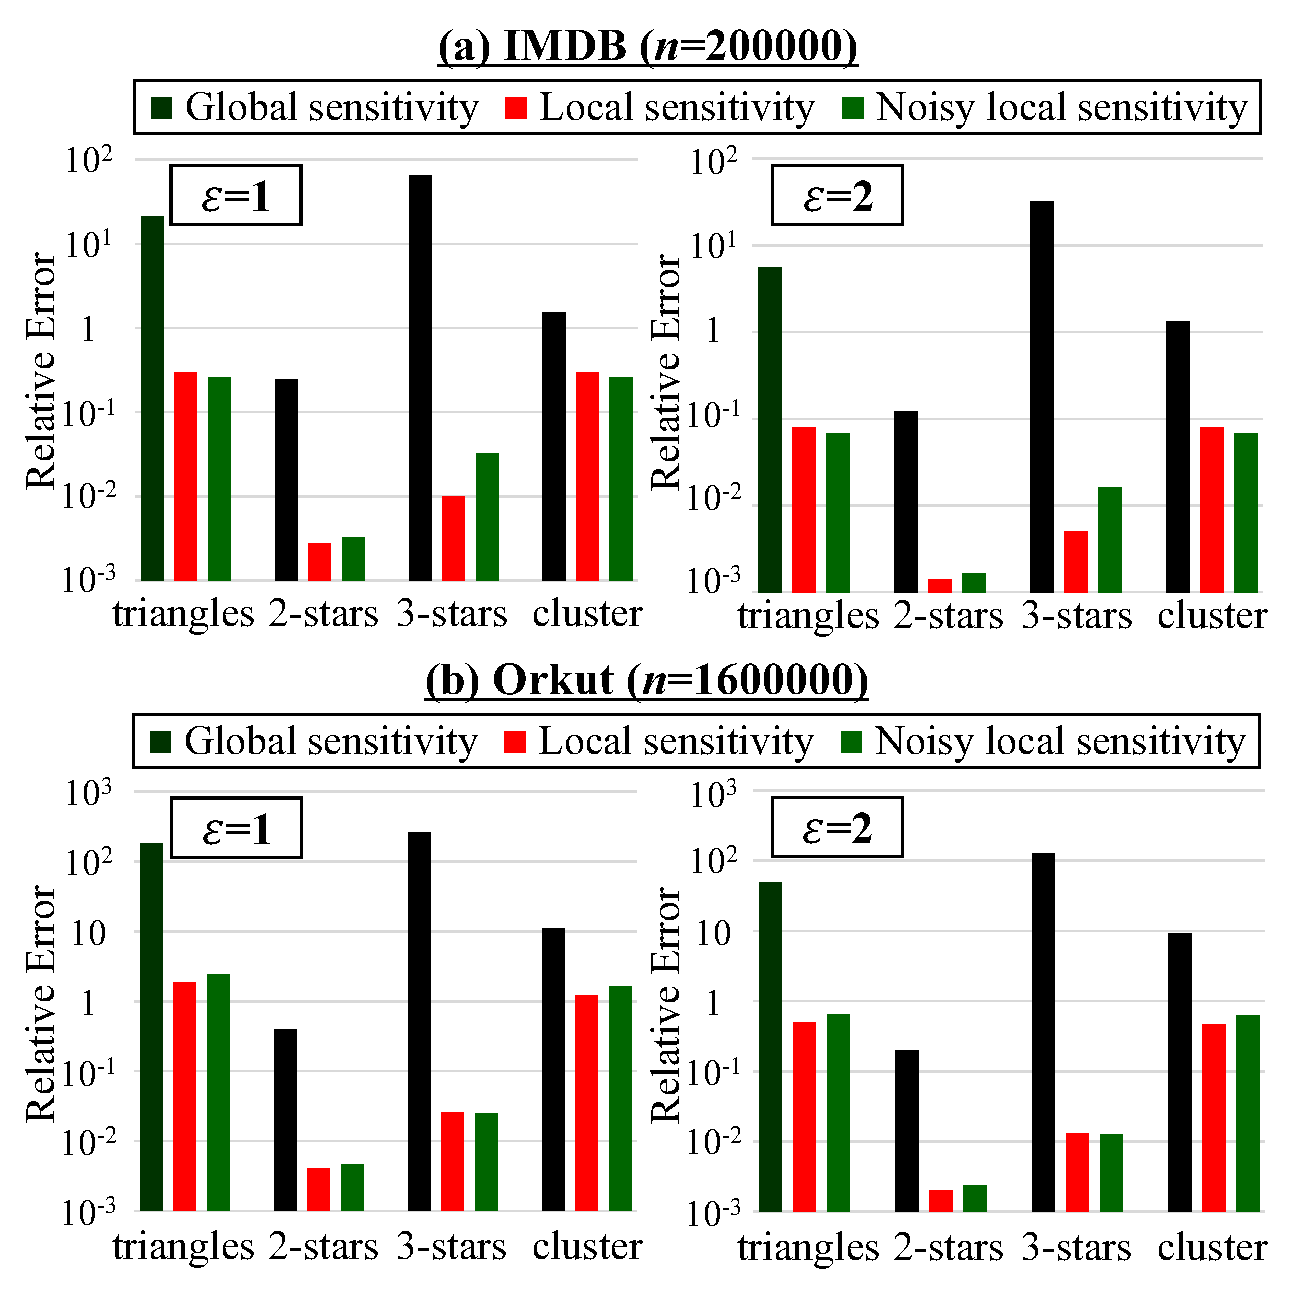
\includegraphics[width=0.99\linewidth]{fig/res4_noisy_local.pdf}
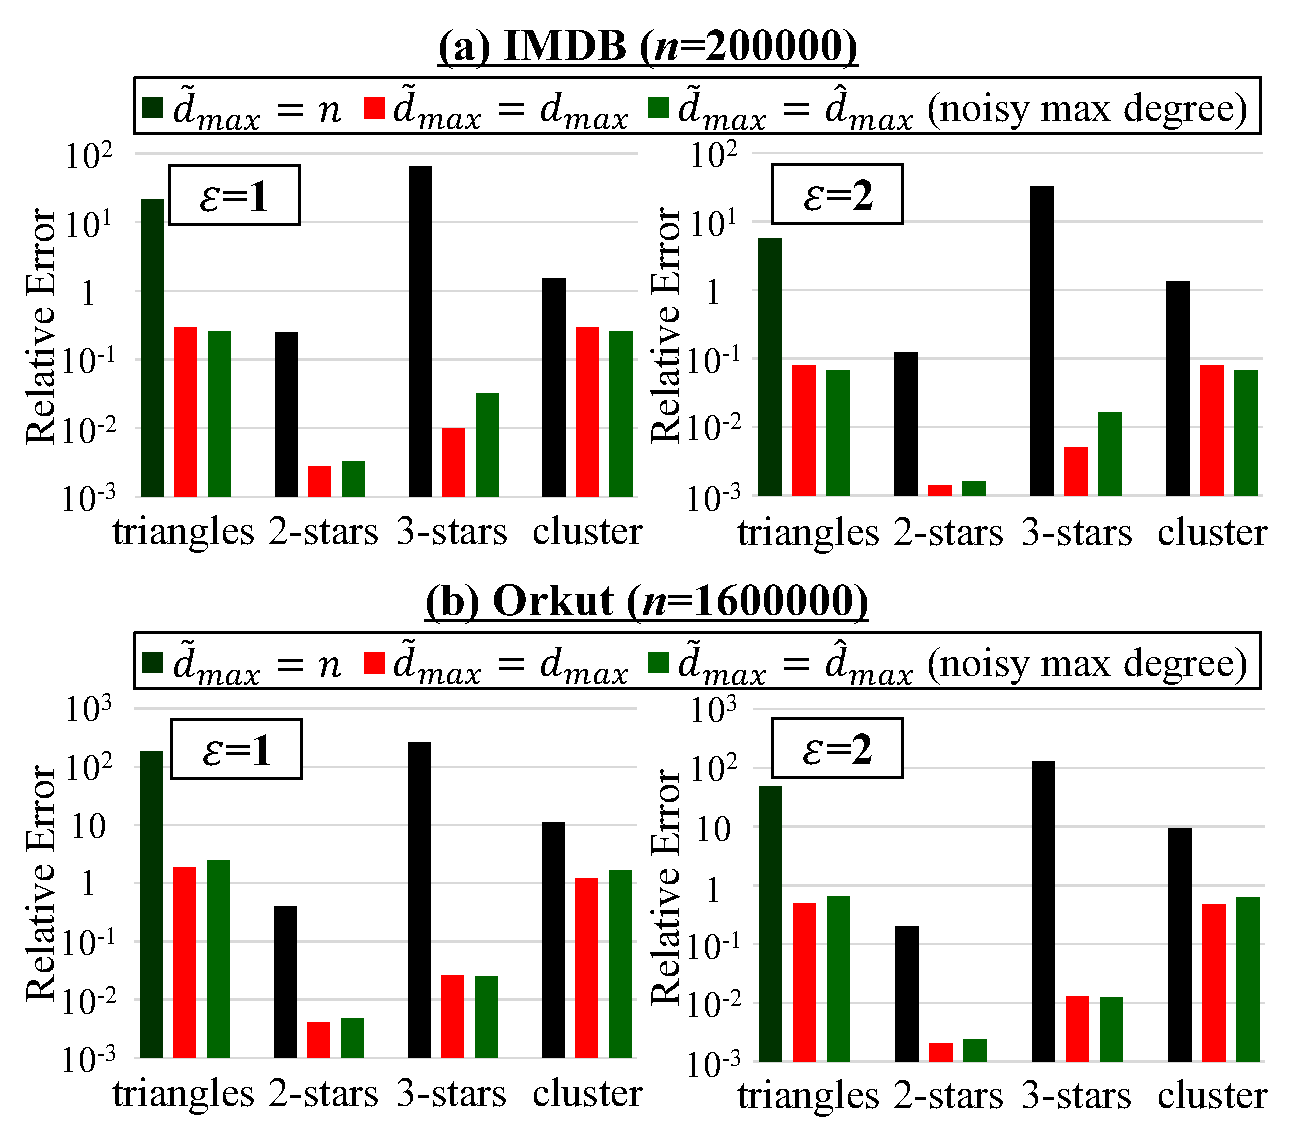
\includegraphics[width=0.99\linewidth]{fig/res4_noisy_max.pdf}

\caption[Relative error when $\td_{max}$ equals \#users, max degree, or noisy max degree.]
{Relative error when $\td_{max} = n$ (\#users), $d_{max}$ (max degree), or $\hd_{max}$ (noisy max degree). 
We used \alg{Local2Rounds$_\triangle$} ($\epsilon = 1$ or $2$) and \alg{LocalLap$_k\star$} ($\epsilon = 1$ or $2$) for estimating triangle counts $f_\triangle(G)$ and $k$-star counts $f_{k\star}(G)$, respectively. 
}
\label{chap1-fig:res4_noisy_local}
\end{figure}

\smallskip
\noindent{\textbf{Private calculation of $d_{max}$.}}~~We have so far assumed that $\td_{max} = d_{max}$ (i.e., $d_{max}$ is publicly available) in our experiments. 
% However, it is difficult for the users and the data collector to know the exact value of $d_{max}$ in advance. 
% Therefore, we 
We 
finally evaluate the methods to privately calculate $d_{max}$ with $\epsilon_0$-edge LDP 
% , which are 
(described in Sections~\ref{chap1-sub:non-interactive_k_stars} and \ref{chap1-sub:two_rounds}). 
% show that even if we privately calculate $d_{max}$ with edge LDP, we can accurately estimate graph statistics in the local model. 

Specifically, we used \alg{Local2Rounds$_\triangle$} and \alg{LocalLap$_k\star$} for estimating $f_\triangle(G)$ and $f_{k\star}(G)$, respectively, and evaluated the following three methods for setting $\td_{max}$: 
% the sensitivity: 
% \begin{enumerate}
%     \item Set $\td_{max} = n$. We call this method the \textit{global sensitivity method} because it results in adding the Laplacian noise with the global sensitivity in Definition~\ref{chap1-def:global_sen}.
%     \item Set $\td_{max} = d_{max}$. We call this method the \textit{local sensitivity method} because it results in adding the Laplacian noise with the local sensitivity. 
% \end{enumerate}
(i) 
% set 
$\td_{max} = n$; 
(ii) 
% set 
$\td_{max} = d_{max}$; 
(iii) 
% set 
$\td_{max} = \hd_{max}$, where $\hd_{max}$ is the private estimate of $d_{max}$ 
% (i.e., 
(noisy max degree) in Sections~\ref{chap1-sub:non-interactive_k_stars} and \ref{chap1-sub:two_rounds}. 
% Note that the first (resp.~second) method results in adding the Laplacian noise with the global (resp.~local) sensitivity without using graph projection. 
% Therefore, we refer to the first method (i) as the \textit{global sensitivity method}, the second method (ii) as the \textit{local sensitivity method}, and the third method (iii) as the \textit{noisy local sensitivity method}. 

We set $n=200000$ in \IMDB{} and $n=1600000$ in \Orkut{}. 
Regarding the total privacy budget $\epsilon$ in edge LDP for estimating $f_\triangle(G)$ or $f_{k\star}(G)$, we set $\epsilon=1$ or $2$. 
We used $\frac{\epsilon}{10}$ for privately calculating $d_{max}$ (i.e., $\epsilon_0 = \frac{\epsilon}{10}$), and the remaining privacy budget $\frac{9\epsilon}{10}$ as input to \alg{Local2Rounds$_\triangle$} or \alg{LocalLap$_k\star$}. 
% estimating $f_\triangle(G)$ or $f_{k\star}(G)$. 
In \alg{Local2Rounds$_\triangle$}, we set $\epsilon_1 = \epsilon_2$; i.e., we set $(\epsilon_0, \epsilon_1, \epsilon_2) = (0.1, 0.45, 0.45)$ or $(0.2, 0.9, 0.9)$. 
% For example, \alg{Local2Rounds$_\triangle$} with $(\epsilon_0, \epsilon_1, \epsilon_2) = (0.1, 0.45, 0.45)$ provides $1$-edge LDP and $1.1$-entire edge LDP (see Section~\ref{chap1-sub:two_rounds}). 
Then we estimated the clustering coefficient in the same way as Figure~\ref{chap1-fig:res3_n_relerr}. 

Figure~\ref{chap1-fig:res4_noisy_local} shows the results. 
Figure~\ref{chap1-fig:res4_noisy_local} shows that 
% the noisy local sensitivity method 
the algorithms with $\td_{max} = \hd_{max}$ (noisy max degree) 
achieves the relative error close to (sometimes almost the same as) 
% the local sensitivity method, 
the algorithms with $\td_{max} = d_{max}$ 
and significantly outperforms 
% the global sensitivity method. 
the algorithms with $\td_{max} = n$. 
This means that we can privately estimate $d_{max}$ without a significant loss of utility. 
% Recall that the private calculation of $d_{max}$ does not increase the number of rounds in \alg{Local2Rounds$_\triangle$}. 
% Therefore, we can privately estimate $d_{max}$ and then accurately estimate all the graph statistics (i.e., triangles, $k$-stars, and the clustering coefficient) within two rounds.

\smallskip
\noindent{\textbf{Summary of results.}}~~In summary, 
% our experimental results were roughly consistent with our theoretical results. 
our experimental results showed that the estimation error of triangle counts is significantly reduced by introducing the interaction between users and a data collector. 
The results also showed that 
% we can accurately estimate graph statistics in the local model. 
% In particular, 
we can achieve small relative errors 
(much smaller than 1) for subgraph counts 
% for a large number of users $n$ 
with privacy budget $\epsilon=1$ or $2$ in edge LDP. 
% The results also showed that we can privately estimate the maximum degree $d_{max}$, which is required in both \alg{Local2Rounds$_\triangle$} and \alg{LocalLap$_k\star$}, without a significant loss of utility. 

As described in Section~\ref{chap1-sec:intro}, non-private 
% triangle or $k$-star 
subgraph 
counts may reveal some friendship information, and a central server may face data breaches. 
Our LDP algorithms are highly beneficial because they enable us to analyze the connection patterns in a graph 
(i.e., subgraph counts) 
or to understand how likely two friends of an individual will also be a friend 
% (which is useful for friend suggestion) 
(i.e., clustering coefficient) 
while strongly protecting individual privacy.
